%Modified from a template provided by Jennifer Pan, August 2011

\documentclass[10pt,letter]{article}
	% basic article document class
	% use percent signs to make comments to yourself -- they will not show up.
\usepackage{pdfsync}
\usepackage{amsmath}
\usepackage{amssymb}
\usepackage{amsthm}
	% packages that allow mathematical formatting

\usepackage{graphicx}
	% package that allows you to include graphics
\graphicspath{ {./images/} }


\usepackage{subcaption}

\usepackage{setspace}
	% package that allows you to change spacing

\onehalfspacing
	% text become 1.5 spaced

\usepackage{fullpage}
% package that specifies normal margins

\usepackage[parfill]{parskip}

\newtheorem*{thm}{Theorem}
\newtheorem{nthm}{Theorem}
\newtheorem{lem}{Lemma}

\begin{document}
	% line of code telling latex that your document is beginning

\title{Problem Set 3}

\author{Katherine Cheng, Richard Davis, Marty Keil}

% \date{Friday April 10, 2015}
	% Note: when you omit this command, the current date is automatically included
 
\maketitle 
	% tells latex to follow your header (e.g., title, author) commands.


\section*{Problem 4: 'Cause I'm Happy}

\paragraph{i)} Statment 2. The only way to make a conditional statement false is if the antecedent is true and the consequent is false. In this case, when the antecedent is true everyone who is a person is happy. If this is true, then it is impossible that there exists a person who is unhappy. 

\paragraph{ii)} Statement 1. The only way to make a conditional statement false is if the antecedent is true and the consequent is false. In this case, when the antecedent is true there is at least one person in the world who is happy. To make the consequent false, we say that not everyone in the world is happy. 

\paragraph{iii)} Statement 2. If we negate this statement we get the formula...

\paragraph{iv)} Statement 2. Take the negation and show that it is always false.

\paragraph{v)} Statement 2. The only way to make an implication false is...

\paragraph{vi)} Statement 2.

\section*{Problem 5: Translating into Logic}

\paragraph{i)}

\paragraph{ii)}

\paragraph{iii)}

\paragraph{iv)}
$\forall Q Set(Q) .\ \exists P Set(P) .\ \forall S Set(S) .\ (S \in P \cap \forall x .\ \forall y .\ (x \in S \rightarrow x \in Q \cap y \not \in S \rightarrow y \not \in Q))$
\paragraph{v)}

\section*{Problem 6: Raven Paradox}
The Raven Paradox involves a scientific statement. As we know from Popper, it is only possible to falsify scientific statements. Induction is a myth.

\section*{Problem 7: Graph Coloring}
Marty can do this.

\section*{Problem 8: Tournament Cycles}
A tournament is a directed graph with $n$ nodes where there is exactly one edge between any pair of distinct nodes and there are no self-loops. Prove that if a tournament graph contains a cycle of any length, then it contains a cycle of length three.

\begin{thm} If a tournament graph contains a cycle of any length, then it contains a cycle of length three.
\end{thm}

\begin{proof} By strong induction. Let $P(n)$ be the statement ``if a tournament contains a cycle of length $n$, then it contains a cycle of length three.'' We will prove that $P(n)$ holds for $n \ge 3$. 

For our base case, we show that $P(3)$ is true. $P(3)$ states that a tournament with a cycle of length 3 contains a cycle of length 3. This is a tautology.

For our inductive step, assume that for some $k \ge 3$ that $P(k)$ is true; that is, that a tournament containing a cycle of length $k$ also contains a cycle of length three. We will prove that $P(k+1)$ is true, that if a tournament contains a cycle of length $k+1$, then it also contains a cycle of length 3.

Consider any tournament with a cycle of length $k+1$. Remove all the edges from this graph except for this cycle. A representation of this graph is shown in Figure \ref{fig:q8_cyc1}. Because this is a tournament, we know that every node must be connected to every other node. 

\begin{figure}
\centering
\begin{minipage}{.5\textwidth}
  \centering
  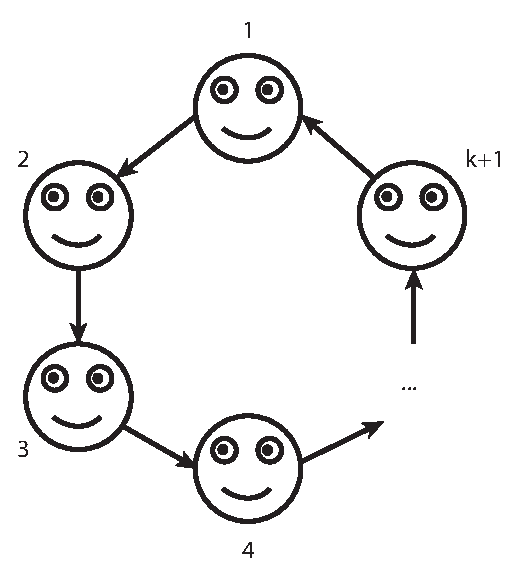
\includegraphics[width=.8\linewidth]{hw3_8_1.eps}
  \captionof{figure}{A figure}
  \label{fig:q8_cyc1}
\end{minipage}%
\begin{minipage}{.5\textwidth}
  \centering
  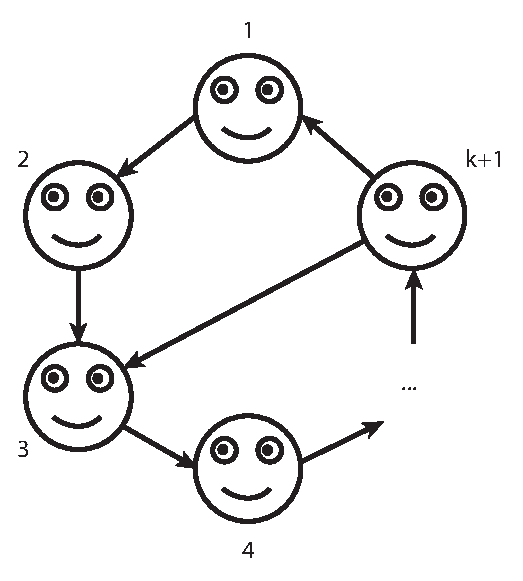
\includegraphics[width=.8\linewidth]{hw3_8_2.eps}
  \captionof{figure}{Another figure}
  \label{fig:q8_test2}
\end{minipage}
\end{figure}

\end{proof}


% \section*{Appendix: Referencing Equations}
% \begin{equation} \label{eq:divbyzero}
%   \frac {1} {0}
% \end{equation}

% This references \ref{eq:divbyzero}.

% \section*{Appendix: Figures in Text}
% Below are two different ways of placing figures side by side in text. The first method creates two sub-figures within a single figure. The second method creates two separate figures.

% \begin{figure}
% \centering
% \begin{minipage}{.5\textwidth}
%   \centering
%   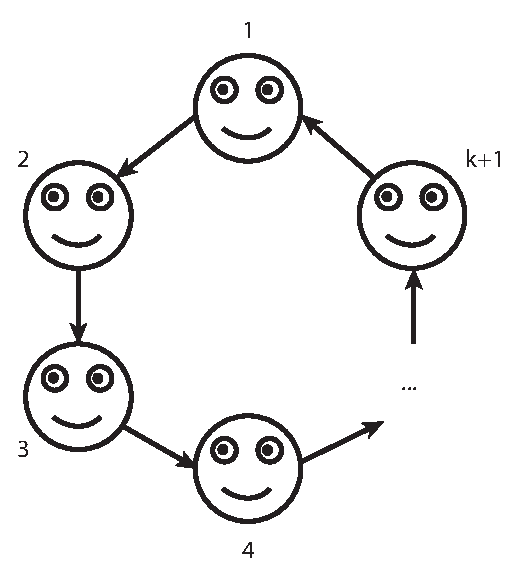
\includegraphics[width=.8\linewidth]{hw3_8_1.eps}
%   \captionof{figure}{A figure}
%   \label{fig:q8_test1}
% \end{minipage}%
% \begin{minipage}{.5\textwidth}
%   \centering
%   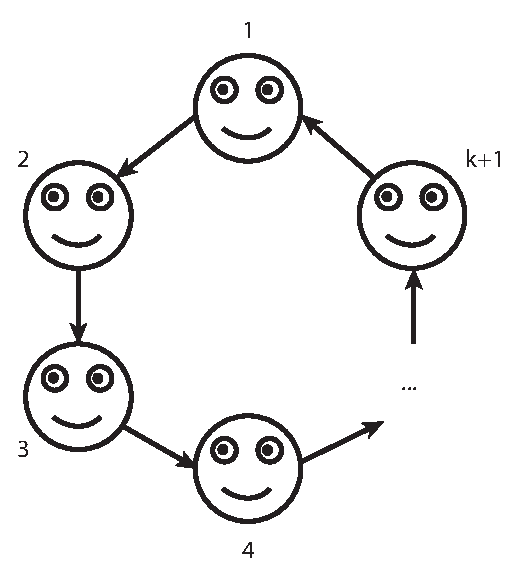
\includegraphics[width=.8\linewidth]{hw3_8_1.eps}
%   \captionof{figure}{Another figure}
%   \label{fig:q8_test2}
% \end{minipage}
% \end{figure}


% \begin{figure}[h]
%   \centering

%   \begin{subfigure}[b]{0.3\textwidth}
%     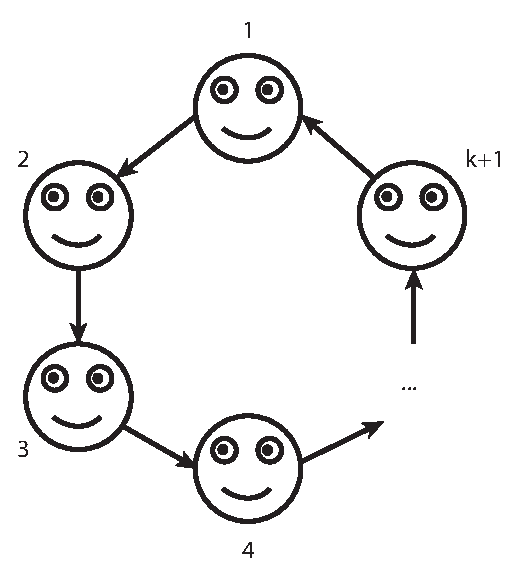
\includegraphics[width=\textwidth]{hw3_8_1.eps}
%     \caption{A cycle with length $k+1$}
%     \label{fig:q8_cycle:a}
%   \end{subfigure}% 
%   \qquad
%   \begin{subfigure}[b]{0.3\textwidth}
%     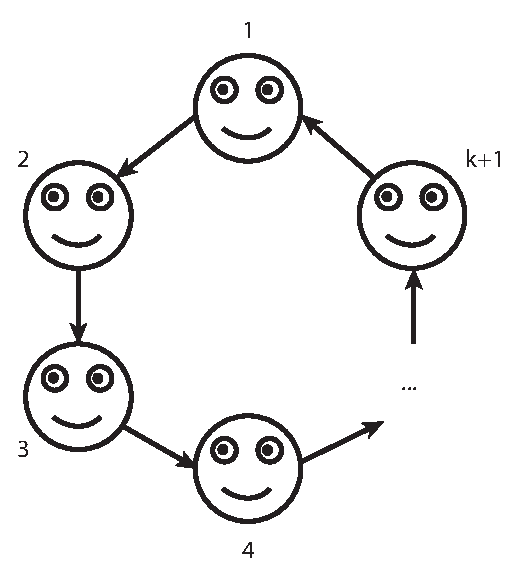
\includegraphics[width=\textwidth]{hw3_8_1.eps}
%     \caption{A cycle with length $k+1$}
%     \label{fig:q8_cycle:b}
%   \end{subfigure}%  

%   \caption{Placeholder}
%   \label{fig:q8}
% \end{figure}

\end{document}
	% line of code telling latex that your document is ending. If you leave this out, you'll get an error

%%% Local Variables:
%%% mode: latex
%%% TeX-master: t
%%% End:
